% =============================================================================
% CHAPTER 3: METHODOLOGY
% =============================================================================

\chapter{METHODOLOGY}
\label{Chapter3}

% -----------------------------------------------------------------------------
\section{Introduction}
\label{sec:ch3intro}
% -----------------------------------------------------------------------------

This chapter formalises the permissiveness problem identified in Chapter~2 and presents the DCA-Trie framework as a solution. We begin by defining the upgraded oracle specification and the Semantic Irrelevance Ratio (SIR), a diagnostic metric that measures constraint quality independently of answer accuracy. We then describe the semantic scoring mechanism shared by both variants, the static pre-filtering design of v1, and the step-wise dynamic expansion design of v2. The chapter closes with the baseline configurations, evaluation protocol, and scope boundaries that govern the experimental work in Chapter~4.

% -----------------------------------------------------------------------------
\section{Formal Problem Specification}
\label{sec:ch3problem}
% -----------------------------------------------------------------------------

\subsection{Restating the Core Limitation of Existing Frameworks}

As established in Chapter~2, current graph-constrained frameworks (notably GCR \citep{luo2025-graph-constrained-reasoning} and DoG \citep{li2024-decoding-on-graphs}) rely on a deterministic oracle that looks only at the fixed graph $\mathcal{G}$ and the starting entities $\mathcal{E}_q$. Regardless of whether the system builds this oracle before decoding or expands it on the fly, the set of valid tokens at any step $t$ remains locked to structural logic:
\begin{equation}
  \mathcal{W}_{\text{val}}^{\text{GCR}}(t) = f(\mathcal{G},\, \mathcal{E}_q)
  \quad \forall\, t
  \label{eq:gcr_oracle}
\end{equation}

By ignoring both the semantic intent of the question $q$ and the reasoning trajectory captured in the prefix $y_{<t}$, this formulation treats every structurally reachable path as equally plausible. In dense, multi-hop Freebase environments, this causes substantial search space inflation. The oracle can admit over 8,000 paths at depth 3, even though only a single path answers the query.

Two separate requirements are in tension here. \textit{Structural validity} ensures the LLM only generates tokens that correspond to real graph edges — current models do this well. \textit{Contextual relevance} ensures the LLM only generates tokens that logically connect to the specific question — current models do not enforce this. The gap between structural compliance and semantic usefulness is the \textit{permissiveness problem}.

\subsection{The Upgraded Oracle Specification}

DCA-Trie addresses this problem by defining a constraint oracle that conditions on both the input question and the evolving generation prefix:
\begin{equation}
  \mathcal{W}_{\text{val}}^{\text{DCA}}(t) = f(\mathcal{G},\, \mathcal{E}_q,\,
  q,\, y_{<t})
  \label{eq:dca_oracle}
\end{equation}
where $q$ is the natural language query and $y_{<t} = (y_1, \ldots, y_{t-1})$ is the generated prefix at step $t$. The upgraded oracle must satisfy three conditions aligned with the project objectives in Chapter~1:

\begin{enumerate}
  \item \textbf{Structural Faithfulness (Condition~F):} Every candidate token $v \in \mathcal{W}_{\text{val}}^{\text{DCA}}(t)$ must correspond to a valid prefix of a path $p \in \mathcal{G}$ at every step $t$. This preserves the 100\% structural faithfulness guarantee achieved by GCR and DoG and prevents ungrounded tokens from entering the valid set.

  \item \textbf{Semantic Relevance Reduction (Condition~R):} The Semantic Irrelevance Ratio (SIR) under DCA-Trie must be lower than the corresponding SIR under GCR when averaged over the evaluation corpus. Using SIR as defined in Section~\ref{sec:ch3sir}:
        \begin{equation}
          \overline{\text{SIR}}\!\left(\mathcal{W}^{\text{DCA}}\right) <
          \overline{\text{SIR}}\!\left(\mathcal{W}^{\text{GCR}}\right)
          \label{eq:sir_condition}
        \end{equation}

  \item \textbf{Recall Preservation (Condition~P):} Semantic pruning must not remove gold paths excessively. The false negative rate (FNR) on the WebQSP validation split must remain below 5\%:
        \begin{equation}
          \text{FNR} = \frac{|\{q \in \mathcal{Q}_{\text{val}} :
          p^*_q \notin \mathcal{W}_{\text{val}}^{\text{DCA}}(t)\}|}{|\mathcal{Q}_{\text{val}}|}
          < 0.05
          \label{eq:fnr}
        \end{equation}
        where $p^*_q$ is the gold path for question $q$ and $\mathcal{Q}_{\text{val}}$ is the held-out 100-question validation set.
\end{enumerate}


% -----------------------------------------------------------------------------
\section{System Architecture Overview}
\label{sec:ch3arch}
% -----------------------------------------------------------------------------

DCA-Trie modifies only the constraint oracle layer of GCR~\citep{luo2025-graph-constrained-reasoning}, leaving the remaining pipeline unchanged. Holding everything else constant means that differences in faithfulness, SIR, and answer accuracy can be attributed directly to the oracle redesign rather than to any other variable. The four layers are as follows:

\begin{enumerate}
  \item \textbf{Entity Linking Layer (Unmodified):} A named entity recognition tool identifies the core query entities $\mathcal{E}_q$ from the raw question $q$. These entities define the starting points for all downstream graph traversal.

  \item \textbf{Constraint Oracle Layer (DCA-Trie Contribution):} This layer governs which tokens the LLM can generate. GCR builds a static prefix tree — a KG-Trie — that includes every path reachable within $L$ hops of the question entities. DCA-Trie replaces this with a semantically filtered oracle: through either static pre-filtering (v1) or step-wise dynamic expansion (v2), no structural edge is admitted to the trie unless it also clears the semantic relevance threshold.

  \item \textbf{Constrained Decoding Layer (Unmodified):} At each autoregressive step, this layer retrieves a binary validity mask from the oracle and applies it to the LLM's logit distribution, setting invalid token probabilities to exactly zero. Every generated token is therefore both structurally grounded and semantically admitted.

  \item \textbf{Inductive Reasoning Layer (Unmodified):} After constrained beam search produces $K$ top reasoning paths, GPT-4o-mini synthesises the final natural language answer from those paths in parallel.
\end{enumerate}

Figure~\ref{fig:architecture} shows the full layout, with the constraint oracle layer highlighted to indicate where the semantic intervention takes place.

\begin{sidewaysfigure}
  \centering
  \resizebox{\textwidth}{!}{%
    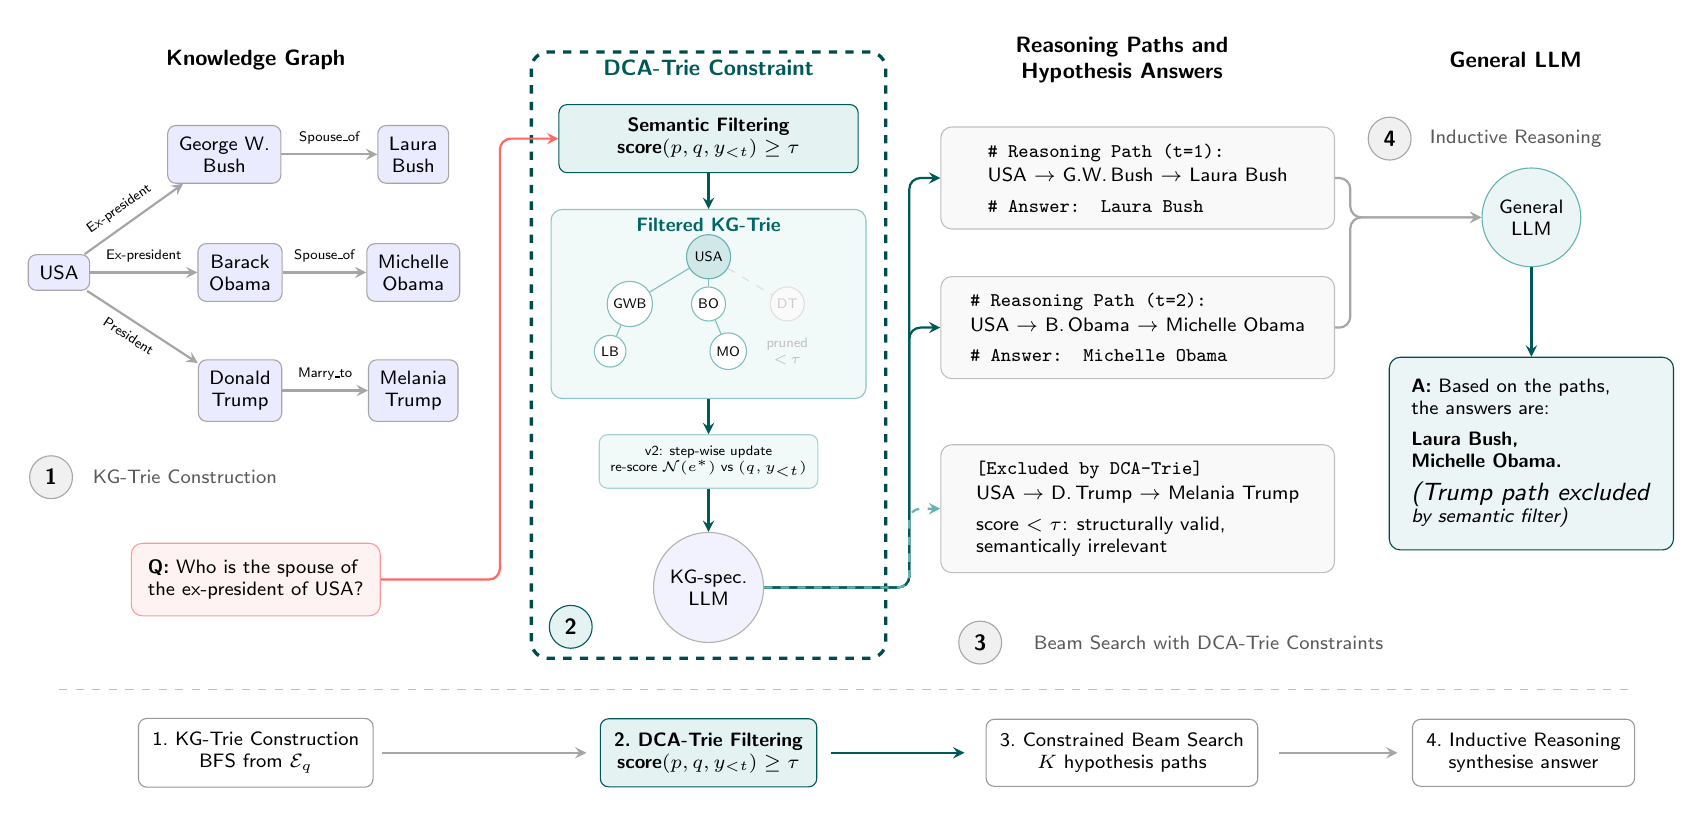
\begin{tikzpicture}[
        >=stealth, font=\sffamily\Large,
        kgnode/.style={draw=gray!70,fill=blue!8,rounded corners=3pt,inner sep=4pt,font=\sffamily\scriptsize,align=center},
        pathbox/.style={draw=gray!50,fill=gray!5,rounded corners=4pt,inner sep=6pt,minimum width=5.0cm,align=left,font=\sffamily\scriptsize},
        filtpath/.style={draw=gray!25,fill=gray!3,rounded corners=4pt,inner sep=6pt,minimum width=5.0cm,align=left,font=\sffamily\scriptsize,text=gray!45},
        ansbox/.style={draw=teal!60!black,fill=teal!8,rounded corners=4pt,inner sep=8pt,minimum width=3.0cm,align=left,font=\sffamily\scriptsize},
        stepbox/.style={draw=black!40,fill=white,rounded corners=3pt,inner sep=5pt,minimum width=2.6cm,minimum height=0.85cm,align=center,font=\sffamily\scriptsize},
        dcabox/.style={draw=teal!70!black,fill=teal!10,rounded corners=3pt,inner sep=5pt,minimum width=2.6cm,minimum height=0.85cm,align=center,font=\sffamily\scriptsize\bfseries},
        llmcirc/.style={circle,draw=gray!60,fill=blue!5,minimum size=1.1cm,align=center,font=\sffamily\scriptsize},
        bigllm/.style={circle,draw=teal!60,fill=teal!8,minimum size=1.25cm,align=center,font=\sffamily\scriptsize},
        arr/.style={->,thick,draw=gray!70},
        rarr/.style={->,thick,draw=red!60},
        tarr/.style={->,thick,draw=teal!70!black},
      ]

      % Knowledge Graph Section
      \node[font=\sffamily\footnotesize\bfseries]at(2.5,0.2){Knowledge Graph};
      \node[kgnode](usa)at(0,-2.5){USA};
      \node[kgnode](gwb)at(2.1,-1.0){George W.\\Bush};
      \node[kgnode](lb)at(4.5,-1.0){Laura\\Bush};
      \node[kgnode](bo)at(2.3,-2.5){Barack\\Obama};
      \node[kgnode](mo)at(4.5,-2.5){Michelle\\Obama};
      \node[kgnode](dt)at(2.3,-4.0){Donald\\Trump};
      \node[kgnode](mt)at(4.5,-4.0){Melania\\Trump};

      \draw[arr](usa)--node[above,sloped,font=\sffamily\tiny,pos=0.45]{Ex-president}(gwb);
      \draw[arr](usa)--node[above,font=\sffamily\tiny,pos=0.5]{Ex-president}(bo);
      \draw[arr](usa)--node[below,sloped,font=\sffamily\tiny,pos=0.45]{President}(dt);
      \draw[arr](gwb)--node[above,font=\sffamily\tiny]{Spouse\_of}(lb);
      \draw[arr](bo)--node[above,font=\sffamily\tiny]{Spouse\_of}(mo);
      \draw[arr](dt)--node[above,font=\sffamily\tiny]{Marry\_to}(mt);

      \node[draw=red!40,fill=red!5,rounded corners=4pt,inner sep=6pt,align=left,
        font=\sffamily\scriptsize,minimum width=2.9cm]
      (qbox)at(2.5,-6.4){\textbf{Q:} Who is the spouse of\\the ex-president of USA?};
      \node[circle,draw=black!35,fill=black!6,font=\sffamily\footnotesize\bfseries,inner sep=3pt]at(-0.1,-5.1){1};
      \node[font=\sffamily\scriptsize,text=black!65,align=center]at(1.6,-5.1){KG-Trie Construction};

      % DCA-Trie Constraint Section
      \draw[draw=teal!60!black,dashed,rounded corners=6pt,line width=1.2pt](6.0,0.3)rectangle(10.5,-7.4);
      \node[font=\sffamily\footnotesize\bfseries,text=teal!70!black]at(8.25,0.1){DCA-Trie Constraint};
      \node[dcabox,minimum width=3.8cm](vf)at(8.25,-0.8){Semantic Filtering\\score$(p,q,y_{<t})\geq\tau$};
      \node[draw=teal!45,fill=teal!5,rounded corners=4pt,minimum width=4.0cm,minimum height=2.4cm](triebox)at(8.25,-2.9){};
      \node[font=\sffamily\scriptsize\bfseries,text=teal!80!black]at(8.25,-1.9){Filtered KG-Trie};

      \node[circle,draw=teal!60,fill=teal!18,inner sep=2pt,font=\sffamily\tiny](tr)at(8.25,-2.3){USA};
      \node[circle,draw=teal!50,fill=white,inner sep=1.5pt,font=\sffamily\tiny](tn1)at(7.25,-2.9){GWB};
      \node[circle,draw=teal!50,fill=white,inner sep=1.5pt,font=\sffamily\tiny](tn2)at(8.25,-2.9){BO};
      \node[circle,draw=gray!25,fill=gray!4,inner sep=1.5pt,font=\sffamily\tiny,text=gray!40](tn3)at(9.25,-2.9){DT};
      \node[circle,draw=teal!50,fill=white,inner sep=1.5pt,font=\sffamily\tiny](tl1)at(7.0,-3.5){LB};
      \node[circle,draw=teal!50,fill=white,inner sep=1.5pt,font=\sffamily\tiny](tl2)at(8.5,-3.5){MO};

      \draw[teal!50,thin](tr)--(tn1); \draw[teal!50,thin](tr)--(tn2);
      \draw[gray!25,thin,dashed](tr)--(tn3);
      \draw[teal!50,thin](tn1)--(tl1); \draw[teal!50,thin](tn2)--(tl2);
      \node[font=\sffamily\tiny,text=gray!50,align=center]at(9.25,-3.5){pruned\\$<\!\tau$};

      \node[draw=teal!35,fill=teal!5,rounded corners=3pt,inner sep=4pt,font=\sffamily\tiny,align=center]
      (upd)at(8.25,-4.9){v2: step-wise update\\re-score $\mathcal{N}(e^{*})$ vs $(q,y_{<t})$};
      \node[llmcirc](kgllm)at(8.25,-6.5){KG-spec.\\LLM};

      \draw[rarr,rounded corners](qbox.east)-- (5.6,-6.4) |- (vf.west);
      \draw[tarr](vf)--(triebox.north);
      \draw[tarr](triebox.south)--(upd.north);
      \draw[tarr](upd)--(kgllm);
      \node[circle,draw=teal!70!black,fill=teal!10,font=\sffamily\footnotesize\bfseries,inner sep=3pt]at(6.5,-7){2};

      % Reasoning Paths and Hypothesis Answers Section
      \node[font=\sffamily\footnotesize\bfseries,align=center]at(13.5,0.2){Reasoning Paths and\\Hypothesis Answers};
      \node[circle,draw=black!35,fill=black!6,font=\sffamily\footnotesize\bfseries,inner sep=3pt]at(11.7,-7.2){3};
      \node[font=\sffamily\scriptsize,text=black!65]at(14.6,-7.2){Beam Search with DCA-Trie Constraints};
      \node[pathbox](p1)at(13.7,-1.3){%
        \texttt{\# Reasoning Path (t=1):}\\[1pt]
        USA $\to$ G.W.\,Bush $\to$ Laura Bush\\[3pt]
        \texttt{\# Answer: Laura Bush}};
      \node[pathbox](p2)at(13.7,-3.2){%
        \texttt{\# Reasoning Path (t=2):}\\[1pt]
        USA $\to$ B.\,Obama $\to$ Michelle Obama\\[3pt]
        \texttt{\# Answer: Michelle Obama}};
      \node[pathbox](p3)at(13.7,-5.5){%
        \texttt{[Excluded by DCA-Trie]}\\[1pt]
        USA $\to$ D.\,Trump $\to$ Melania Trump\\[3pt]
        score $<\tau$: structurally valid,\\
        semantically irrelevant};

      \draw[tarr,rounded corners](kgllm.east)-- (10.8,-6.5) |- (p1.west);
      \draw[tarr,rounded corners](kgllm.east)-- (10.8,-6.5) |- (p2.west);
      \draw[tarr,dashed,draw=teal!60,rounded corners](kgllm.east)-- (10.8,-6.5) |- (p3.west);

      % General LLM Section
      \node[font=\sffamily\footnotesize\bfseries]at(18.5,0.2){General LLM};
      \node[bigllm](gllm)at(18.7,-1.8){General\\LLM};
      \node[ansbox](ans)at(18.7,-4.8){%
        \textbf{A:} Based on the paths,\\
        the answers are:\\[3pt]
        \textbf{Laura Bush,}\\
        \textbf{Michelle Obama.}\\[4pt]
        \small\textit{(Trump path excluded}\\
        \textit{by semantic filter)}};
      \node[circle,draw=black!35,fill=black!6,font=\sffamily\footnotesize\bfseries,inner sep=3pt]at(16.9,-0.8){4};
      \node[font=\sffamily\scriptsize,text=black!65]at(18.5,-0.8){Inductive Reasoning};

      \draw[arr,rounded corners](p1.east) -| (16.4,-1.8) -- (gllm.west);
      \draw[arr,rounded corners](p2.east) -| (16.4,-1.8) -- (gllm.west);
      \draw[tarr](gllm)--(ans);

      % Footer Steps Section
      \draw[gray!50,dashed](0,-7.8)--(20.0,-7.8);
      \node[stepbox]at(2.5,-8.6){1.\ KG-Trie Construction\\BFS from $\mathcal{E}_q$};
      \node[dcabox]at(8.25,-8.6){2.\ DCA-Trie Filtering\\score$(p,q,y_{<t})\geq\tau$};
      \node[stepbox]at(13.5,-8.6){3.\ Constrained Beam Search\\$K$ hypothesis paths};
      \node[stepbox]at(18.6,-8.6){4.\ Inductive Reasoning\\synthesise answer};

      \draw[arr](4.1,-8.6)--(6.7,-8.6);
      \draw[tarr](9.8,-8.6)--(11.5,-8.6);
      \draw[arr](15.5,-8.6)--(17.0,-8.6);
    \end{tikzpicture}
  }%
  \caption[DCA-Trie System Architecture]{DCA-Trie System Architecture.}
  \label{fig:architecture}
\end{sidewaysfigure}

% -----------------------------------------------------------------------------
\section{The Semantic Irrelevance Ratio: Definition and Measurement}
\label{sec:ch3sir}
% -----------------------------------------------------------------------------

\subsection{Motivation}

Standard performance markers for knowledge graph decoding — Hits@1, F1, structural faithfulness — evaluate the final output rather than the mechanism that produced it. A model may reach the correct gold path while spending most of its search on structurally valid but semantically irrelevant alternatives. Without a dedicated metric, it is impossible to tell whether one oracle is more focused than another independently of answer quality. SIR fills this gap: it measures how much of the admitted path space is semantically irrelevant, giving a direct handle on oracle permissiveness that is orthogonal to accuracy.

\subsection{Formal Definition of SIR}

Suppose $\mathcal{P}(q, t)$ represents all paths that the constraint oracle allows at decoding step $t$ for question $q$. A candidate path $p \in \mathcal{P}(q, t)$ fails the semantic stringency test if its contextual similarity drops below a fixed reference threshold $\tau_{\text{ref}}$:
\begin{equation}
  \text{irrelevant}(p, q, y_{<t}) = \mathbf{1}\!\left[
    \cos\!\bigl(E(p),\; E(\text{concat}(q, y_{<t}))\bigr) < \tau_{\text{ref}}
    \right]
  \label{eq:irrelevant}
\end{equation}
where $E(\cdot)$ is the \texttt{all-MiniLM-L6-v2} sentence encoder and $\tau_{\text{ref}} = 0.3$ is a fixed reference threshold. This reference threshold is intentionally separate from DCA-Trie's admission threshold $\tau$ and is not tuned.

The step-level SIR for question $q$ at decoding step $t$ is then:
\begin{equation}
  \text{SIR}(q, t) = \frac{\sum_{p \in \mathcal{P}(q,t)}
    \text{irrelevant}(p, q, y_{<t})}{|\mathcal{P}(q, t)|}
  \label{eq:sir_step}
\end{equation}

Corpus-level SIR is computed by averaging over all questions and all valid decoding steps up to depth $L$:
\begin{equation}
  \overline{\text{SIR}} = \frac{1}{|\mathcal{Q}|} \sum_{q \in \mathcal{Q}}
  \frac{1}{L_q} \sum_{t=1}^{L_q} \text{SIR}(q, t)
  \label{eq:sir_aggregate}
\end{equation}
where $L_q$ is the hop length of the generated reasoning chain for question $q$.

\subsection{Properties and Interpretation}

By definition, $\overline{\text{SIR}} \in [0,1]$. A value near 1 indicates that most admitted paths are irrelevant — the model faces a large, noisy search space and must resolve it internally. A value near 0 indicates that the constraint set is tightly aligned with question semantics. GCR and DoG tend toward high SIR, particularly at larger hop depths where path counts grow exponentially. DCA-Trie targets lower SIR by filtering semantically weak paths while retaining structurally valid ones. Results are reported by hop depth to show how this effect scales with reasoning complexity.

% -----------------------------------------------------------------------------
\section{Semantic Relevance Scoring Mechanism}
\label{sec:ch3scorer}
% -----------------------------------------------------------------------------

\subsection{Scorer Architecture}

The semantic relevance scorer implements the transition from a static oracle $f(\mathcal{G}, \mathcal{E}_q)$ to a context-aware oracle $f(\mathcal{G}, \mathcal{E}_q, q, y_{<t})$. As illustrated in Figure~\ref{fig:scorer}, it takes a candidate KG path $p$, the question $q$, and the partial generation $y_{<t}$, and returns a relevance score in $[0,1]$.

A path $p = (e_0, r_1, e_1, \ldots, r_L, e_L)$ is serialized into a text sequence:
\begin{equation}
  \text{str}(p) = e_0 \;\|\; r_1 \;\|\; e_1 \;\|\; \cdots \;\|\; r_L \;\|\; e_L
  \label{eq:pathstr}
\end{equation}
where entity IDs are mapped to readable Freebase names when available, and relation strings are normalised (e.g., underscore replacement). The query-side context is serialized as:
\begin{equation}
  \text{query}(q, y_{<t}) = q \;\|\; \texttt{[SEP]} \;\|\;
  \text{str}(y_{<t})
  \label{eq:querystr}
\end{equation}
where $\text{str}(y_{<t})$ is the detokenised generation prefix.

\begin{figure}[H]
  \centering
  \begin{tikzpicture}[
    box/.style={draw, rounded corners, minimum width=2.5cm, minimum height=0.8cm, align=center, font=\small},
    encoder/.style={draw, fill=blue!10, rounded corners, minimum width=2.5cm, minimum height=0.8cm, align=center, font=\small},
    arrow/.style={-{Stealth[scale=1]}, thick},
    node distance=1.5cm
    ]

    % Inputs
    \node[box] (query) {Question $q$ \\ + Context $y_{<t}$};
    \node[box, right=2cm of query] (path) {Candidate Path $p$};

    % Formatter
    \node[box, below=1cm of query] (qformat) {String Formatter\\(Eq 3.9)};
    \node[box, below=1cm of path] (pformat) {String Formatter\\(Eq 3.8)};

    % Encoders
    \node[encoder, below=1cm of qformat] (qenc) {Sentence Encoder\\(MiniLM)};
    \node[encoder, below=1cm of pformat] (penc) {Sentence Encoder\\(MiniLM)};

    % Cosine
    \node[box, diamond, aspect=2, below=1cm of $(qenc)!0.5!(penc)$] (cos) {Cosine\\Similarity};

    % Threshold
    \node[box, below=1cm of cos] (thresh) {Admit if \\ $s \geq \tau$};

    % Connections
    \draw[arrow] (query) -- (qformat);
    \draw[arrow] (path) -- (pformat);

    \draw[arrow] (qformat) -- node[left, font=\footnotesize] {Query str} (qenc);
    \draw[arrow] (pformat) -- node[right, font=\footnotesize] {Path str} (penc);

    \draw[arrow] (qenc) -- node[left, font=\footnotesize] {Vector $\mathbf{u}$} (cos);
    \draw[arrow] (penc) -- node[right, font=\footnotesize] {Vector $\mathbf{v}$} (cos);

    \draw[arrow] (cos) -- node[right, font=\footnotesize] {Score $s$} (thresh);
  \end{tikzpicture}
  \caption[Semantic Relevance Scoring Mechanism]{Semantic Relevance Scoring Mechanism.}
  \label{fig:scorer}
\end{figure}

Both $\text{str}(p)$ and $\text{query}(q, y_{<t})$ are encoded using \texttt{all-MiniLM-L6-v2} \citep{reimers2019sbert} into 384-dimensional vectors. Relevance is computed as cosine similarity:
\begin{equation}
  \text{score}(p,\, q,\, y_{<t}) = \cos\!\bigl(
  E\!\left(\text{str}(p)\right),\;\;
  E\!\left(\text{query}(q, y_{<t})\right)
  \bigr)
  \label{eq:scorer}
\end{equation}

A candidate path is admitted into $\mathcal{W}_{\text{val}}^{\text{DCA}}(t)$ if and only if $\text{score}(p, q, y_{<t}) \geq \tau$, where $\tau$ is the admission threshold. This binary decision integrates the semantic score directly into the logit-masking framework.

\subsection{Threshold Selection}

The admission threshold $\tau$ is tuned on a separate 100-question WebQSP validation split. Selection prioritises Condition~P (low false negatives) while maximising trie reduction relative to GCR. We sweep $\tau \in [0.1, 0.6]$ with step size 0.05 and select the highest value satisfying $\text{FNR} < 0.05$. Thresholds are tuned independently for v1 and v2, since v2 uses step-wise context updates and therefore follows a different pruning dynamic.

\subsection{Encoder Caching}

To reduce redundant computation during beam search, path embeddings $E(\text{str}(p))$ are cached. In v1, caching is done upfront because the trie is fixed after construction. In v2, embeddings are cached lazily as new branches are expanded. The query-context embedding $E(\text{query}(q, y_{<t}))$, by contrast, must be recomputed whenever the generation prefix changes.

% -----------------------------------------------------------------------------
\section{DCA-Trie v1: Static Semantic Filtering}
\label{sec:ch3v1}
% -----------------------------------------------------------------------------

\subsection{Design Rationale}

DCA-Trie v1 targets the permissiveness problem while preserving the efficient static-trie design of GCR. The key observation is that many structurally reachable paths are semantically unrelated to the question, and this can be determined before decoding begins — using only $q$, without needing any generated context. Scoring all candidate paths against the question during preprocessing and discarding those below $\tau$ reduces the search space once, permanently, before autoregressive generation starts. Figure~\ref{fig:v1} summarises this offline filtering workflow.

\begin{figure}[H]
  \centering
  \resizebox{0.45\textwidth}{!}{%
    \begin{tikzpicture}[
      box/.style={draw, rounded corners, minimum width=2.9cm, minimum height=0.95cm, align=center, font=\small},
      db/.style={draw, cylinder, shape border rotate=90, aspect=0.25, minimum width=2.9cm, minimum height=1.25cm, align=center, font=\small, fill=gray!10},
      arrow/.style={-{Stealth[scale=1]}, thick},
      node distance=1.0cm
      ]

      \node[box] (query) {Question $q$};
      \node[db, right=2.5cm of query] (kg) {Knowledge\\Graph $\mathcal{G}$};

      \node[box, below=0.87cm of query] (qenc) {Precompute\\Query Vector $\mathbf{u}$};
      \node[box, below=0.87cm of kg] (bfs) {BFS Enumeration\\(Max $L$ hops)};

      \node[box, below=0.87cm of bfs] (paths) {Candidate Paths $\mathcal{P}$};

      \node[box, fill=teal!10, below=1cm of paths, xshift=-2.2cm, text width=8.2cm, align=left, minimum height=3.0cm] (filter) {\centering\textbf{Semantic Filter Loop}\\[2pt]
        \raggedright For each $p \in \mathcal{P}$:\\
        1. Compute $\mathbf{v}_p \leftarrow E(\text{str}(p))$\\
        2. Compute $s_p \leftarrow \cos(\mathbf{u}, \mathbf{v}_p)$\\
        3. Keep $p$ if $s_p \geq \tau$};

      \node[box, below=1.1cm of filter] (trie) {Construct Filtered\\KG-Trie $\mathcal{T}^{\text{v1}}$};

      \draw[arrow] (query) -- (qenc);
      \draw[arrow] (kg) -- (bfs);
      \draw[arrow] (bfs) -- (paths);

      \draw[arrow] (qenc.south) -- ([xshift=-3.2cm]filter.north);
      \draw[arrow] (paths.south) -- ([xshift=2.2cm]filter.north);

      \draw[arrow] (filter) -- node[right, font=\footnotesize] {$\mathcal{P}_{\text{filtered}}$} (trie);
    \end{tikzpicture}
  }%
  \caption[Static Semantic Filtering Pipeline (DCA-Trie v1)]{Static Semantic Filtering Pipeline for DCA-Trie v1.}
  \label{fig:v1}
\end{figure}

\subsection{Algorithm for DCA-Trie v1}

\begin{algorithm}[H]
  \caption{DCA-Trie v1: Static Semantic Filtering at Construction Time}
  \label{alg:v1}
  \small
  \begin{algorithmic}[1]
    \Require Knowledge graph $\mathcal{G}$; question entities $\mathcal{E}_q$;
    question $q$; max hop depth $L$; admission threshold $\tau$;
    sentence encoder $E$
    \Ensure Semantically filtered KG-Trie $\mathcal{T}^{\text{v1}}$

    \State \textbf{Precompute query embedding:}
    $\mathbf{u} \gets E(\text{query}(q, \varepsilon))$
    \Comment{$y_{<t} = \varepsilon$ at construction time}

    \State \textbf{Enumerate paths:}
    $\mathcal{P} \gets \textsc{BFS}(\mathcal{G}, \mathcal{E}_q, L)$
    \Comment{All paths within $L$ hops, as in GCR}

    \State \textbf{Score and filter:}
    \For{each path $p \in \mathcal{P}$}
    \State $\mathbf{v}_p \gets E(\text{str}(p))$
    \Comment{Precompute and cache path embedding}
    \State $s_p \gets \cos(\mathbf{u}, \mathbf{v}_p)$
    \If{$s_p \geq \tau$}
    \State Add $p$ to $\mathcal{P}_{\text{filtered}}$
    \EndIf
    \EndFor

    \State \textbf{Construct filtered trie:}
    $\mathcal{T}^{\text{v1}} \gets \textsc{BuildTrie}(\mathcal{P}_{\text{filtered}})$

    \State \Return $\mathcal{T}^{\text{v1}}$
  \end{algorithmic}
\end{algorithm}

Algorithm~\ref{alg:v1} runs in two phases that are cleanly separated: an offline filtering phase and an online generation phase. The offline phase (lines 1--5) is a single pass over all BFS-enumerated paths, scoring each against the pre-computed query embedding and retaining only those that clear $\tau$. The resulting filtered trie $\mathcal{T}^{\text{v1}}$ is then fixed for the rest of generation. Semantic selectivity is therefore a one-time cost: the online decoding phase queries the same static structure that GCR uses, with no additional per-step overhead beyond trie lookup.

\subsection{Complexity Analysis}

Building $\mathcal{T}^{\text{v1}}$ has an offline cost of $O(|\mathcal{P}| \cdot d_E)$, where $|\mathcal{P}|$ is the number of BFS-enumerated paths and $d_E = 384$ is the embedding dimension. This is a one-time preprocessing cost. During decoding, lookup complexity is $O(d)$, matching GCR, because child lookup in the trie is constant-time. Memory scales as $O(|\mathcal{P}_{\text{filtered}}| \cdot L)$, typically much smaller than GCR's $O(|\mathcal{P}| \cdot L)$ because semantic filtering removes the majority of structurally reachable but semantically irrelevant paths.

\subsection{Faithfulness Guarantee}

DCA-Trie v1 maintains structural faithfulness by design. Every path retained in $\mathcal{P}_{\text{filtered}}$ originates from $\textsc{BFS}(\mathcal{G}, \mathcal{E}_q, L)$, ensuring that each triplet $(e_{i-1}, r_i, e_i)$ is a valid graph edge. Semantic filtering removes paths; it does not introduce new tokens or edges. Any token passed through $\mathcal{T}^{\text{v1}}$ therefore remains structurally grounded, satisfying Condition~F, provided that token-mask construction and tokenizer alignment are correct.

% -----------------------------------------------------------------------------
\section{DCA-Trie v2: Step-Wise Dynamic Expansion}
\label{sec:ch3v2}
% -----------------------------------------------------------------------------

\subsection{Design Rationale}

DCA-Trie v2 implements the full dynamic oracle in Equation~\eqref{eq:dca_oracle} by conditioning constraints on the evolving prefix $y_{<t}$. The key motivation is that question-level intent, used alone in v1, may not be sufficient as reasoning progresses: after the model has committed to \textit{Elvis\_Presley $\to$ starred\_in $\to$ Blue\_Hawaii}, plausible next expansions should focus on facts about \textit{Blue\_Hawaii} specifically, not on the original entity set. The relevant neighbourhood shifts with each committed entity, and a static trie cannot capture that shift.

Architecturally, v2 follows the step-wise traversal pattern of DoG~\citep{li2024-decoding-on-graphs} but adds semantic gating to each local expansion. After each committed entity $e_t$, the trie expands only to structurally valid neighbours that also satisfy threshold $\tau$ against the updated context:
\begin{equation}
  \mathcal{T}_{t+1} = \mathcal{T}_t \;\cup\; \bigl\{(e_t,\, r,\, e') :
  (e_t, r, e') \in \mathcal{T}_{\mathcal{G}} \;\wedge\;
  \text{score}(e', q, y_{<t}) \geq \tau\bigr\}
  \label{eq:v2expansion}
\end{equation}
where $\mathcal{T}_{\mathcal{G}}$ is the set of graph triplets. The distinction from DoG is not \textit{when} expansion happens but \textit{how} candidates are admitted: each step is both graph-valid and semantically gated. The full workflow is shown in Figure~\ref{fig:v2}.

\begin{figure}[H]
  \centering

  \begin{tikzpicture}[
    box/.style={draw, rounded corners, minimum width=2.5cm, minimum height=0.8cm, align=center, font=\small},
    db/.style={draw, cylinder, shape border rotate=90, aspect=0.25, minimum width=2.5cm, minimum height=1.2cm, align=center, font=\small, fill=gray!10},
    arrow/.style={-{Stealth[scale=1]}, thick},
    node distance=1.2cm
    ]

    \node[box] (step) {Decoding Step $t$\\with partial $y_{<t}$};
    \node[box, below=1cm of step] (llm) {LLM calculates\\logits for $y_t$};
    \node[box, right=1.5cm of step] (trie) {Current KG-Trie $\mathcal{T}_{t-1}$};

    \node[box, below=1cm of trie] (lookup) {Lookup Valid\\Tokens $\mathcal{V}_t$};

    \node[box, fill=purple!10, below=1.5cm of $(llm)!0.5!(lookup)$] (mask) {Logit Masking\\(Eq 2.2)};

    \node[box, below=1cm of mask] (commit) {Commit Entity $e_t$};

    \node[box, fill=teal!10, text width=7cm, right=2.5cm of mask] (expand) {\textbf{Dynamic Semantic Expansion}\\1. $\mathbf{u}_t \leftarrow E(\text{query}(q, y_{\leq t}))$\\2. For each $(e_t, r, e') \in \mathcal{T}_{\mathcal{G}}$:\\ \quad \quad if $\cos(\mathbf{u}_t, \mathbf{v}_{e'}) \geq \tau$,\\ \quad \quad add $(e_t, r, e')$ to $\mathcal{T}_t$};

    \draw[arrow] (step) -- (llm);
    \draw[arrow] (trie) -- (lookup);
    \draw[arrow] (llm) -- (mask);
    \draw[arrow] (lookup) -- (mask);
    \draw[arrow] (mask) -- node[left, font=\footnotesize] {Sample $y_t$} (commit);

    \draw[arrow] (commit) -| node[pos=0.25, below, font=\footnotesize] {Trigger Expansion} (expand);
    \draw[arrow] (expand) |- node[pos=0.75, above, font=\footnotesize] {Update to $\mathcal{T}_t$} (trie);
  \end{tikzpicture}
  \caption[Step-Wise Dynamic Expansion Workflow (DCA-Trie v2)]{Step-Wise Dynamic Expansion Workflow for DCA-Trie v2.}
  \label{fig:v2}
\end{figure}

\newpage

\subsection{Algorithm for DCA-Trie v2}

\begin{algorithm}[H]
  \caption{DCA-Trie v2: Step-Wise Semantic Expansion}
  \label{alg:v2}
  \small
  \begin{algorithmic}[1]
    \Require Knowledge graph $\mathcal{G}$; question entities $\mathcal{E}_q$;
    question $q$; admission threshold $\tau$; sentence encoder $E$;
    LLM with vocabulary $\mathcal{V}$
    \Ensure Generated reasoning chain $y_1 \ldots y_T$

    \State \textbf{Initialize trie} with entity nodes for $\mathcal{E}_q$:
    $\mathcal{T}_0 \gets \{e_q : e_q \in \mathcal{E}_q\}$

    \State \textbf{Precompute query embedding:}
    $\mathbf{u}_0 \gets E(\text{query}(q, \varepsilon))$

    \For{each step $t = 1$ \textbf{to} $T$}
    \State $\mathcal{V}_t \gets \textsc{TrieLookup}(\mathcal{T}_{t-1}, y_{<t})$
    \Comment{Valid tokens from current trie}
    \State $\mathbf{m}_t[v] \gets \mathbf{1}[v \in \mathcal{V}_t]$ for all $v$
    \State $\tilde{\boldsymbol{\alpha}}_t \gets \mathbf{m}_t \odot
      \textsc{LLMLogits}(y_{<t}, x)$
    \State $y_t \gets \text{beam-search-step}(\tilde{\boldsymbol{\alpha}}_t)$

    \If{$y_t$ is an \textit{entity} token $e_t$}
    \Comment{Expansion triggered at entity commits}
    \State \textbf{Update query embedding:}
    $\mathbf{u}_t \gets E(\text{query}(q, y_{\leq t}))$
    \State \textbf{Expand trie:}
    \For{each $(e_t, r, e') \in \mathcal{T}_{\mathcal{G}}$}
    \State $\mathbf{v}_{e'} \gets E(\text{str}((e_t, r, e')))$
    \Comment{Cache if previously computed}
    \State $s \gets \cos(\mathbf{u}_t, \mathbf{v}_{e'})$
    \If{$s \geq \tau$}
    \State Add $(e_t, r, e')$ to $\mathcal{T}_t$
    \EndIf
    \EndFor
    \Else
    \State $\mathcal{T}_t \gets \mathcal{T}_{t-1}$
    \Comment{No expansion at relation token steps}
    \EndIf
    \EndFor
    \State \Return $y_1 \ldots y_T$
  \end{algorithmic}
\end{algorithm}

The key structural difference from v1 is in lines 8--15 of Algorithm~\ref{alg:v2}. Expansion is triggered only when the model commits an entity token, not at every step. At that moment, the query embedding is updated to incorporate $y_{\leq t}$ — the full reasoning path so far — before scoring the candidate neighbours. This means the semantic filter at step $t$ is asking a different, more specific question than at step 1: not ``does this path relate to the question?'' but ``does this neighbour continue the path the model has already taken, in the direction the question requires?'' At relation-token steps, the trie is held constant and no encoder calls are made. This design concentrates computation where it matters most, at entity decision points, while keeping per-step overhead predictable.

% -----------------------------------------------------------------------------
\section{Baseline Systems}
\label{sec:ch3baseline}
% -----------------------------------------------------------------------------

Four system configurations are evaluated to isolate the contribution of DCA-Trie's oracle design:

\textbf{CoT Baseline:} The same Llama-3.1-8B model~\citep{dubey2024llama3} used in GCR, run without any KG constraint oracle and prompted with standard chain-of-thought reasoning. This is the unconstrained reference point.

\textbf{GCR:} The original Graph-Constrained Reasoning framework~\citep{luo2025-graph-constrained-reasoning} with static KG-Trie constraints $\mathcal{W}_{\text{val}}(t)=f(\mathcal{G},\mathcal{E}_q)$. The primary constrained baseline; reproduction targets WebQSP Hits@1 within 1--2\% of the published 92.6\%.

\textbf{DCA-Trie v1:} The static semantic filtering variant described in Section~\ref{sec:ch3v1}, implemented as a preprocessing step in the GCR pipeline with validation-calibrated threshold $\tau$.

\textbf{DCA-Trie v2:} The dynamic step-wise expansion variant described in Section~\ref{sec:ch3v2}, integrated into the decoding loop.

All configurations use the same Llama-3.1-8B backbone, the same entity-linking pipeline for $\mathcal{E}_q$, and matched beam width ($k=5$ for constrained systems). Any observed differences therefore reflect oracle design rather than model or preprocessing variation.

% -----------------------------------------------------------------------------
\section{Evaluation Protocol}
\label{sec:ch3eval}
% -----------------------------------------------------------------------------

\subsection{Datasets}

Evaluation is conducted on two standard Freebase-based KGQA datasets~\citep{bollacker2008freebase}:

\textbf{WebQSP}~\citep{yih2016websqp}: 4,737 questions, mostly requiring 1--2 hops. The standard test set is used for evaluation. A separate disjoint set of 100 questions is reserved solely for threshold calibration.

\textbf{ComplexWebQuestions (CWQ)}~\citep{talmor2018cwq}: 34,689 questions with higher compositional complexity and hop depths up to 4. Used in full for evaluation with no overlap with the calibration split.

\subsection{Evaluation Metrics}

Five metrics are computed across both datasets:

\begin{enumerate}
  \item \textbf{Hits@1:} The proportion of examples where the top predicted answer matches the gold entity.

  \item \textbf{F1:} Entity-level overlap score for settings with multiple acceptable answers, following standard KGQA practice~\citep{lan2022survey}.

  \item \textbf{Structural Faithfulness Rate:} The fraction of generated paths where all triplets are verified in the underlying KG.

  \item \textbf{Semantic Irrelevance Ratio (SIR):} Computed using Equations~\eqref{eq:sir_step} and \eqref{eq:sir_aggregate} with fixed reference threshold $\tau_{\text{ref}}=0.3$.

  \item \textbf{Average Trie Size Per Step:} The mean size of the valid token set $|\mathcal{V}_t|$ across decoding steps, a direct indicator of constraint selectivity.
\end{enumerate}

\subsection{Hop-Depth Stratification}

All major metrics (except binary structural faithfulness) are reported by hop depth (1, 2, 3, and 4), consistent with prior KGQA analysis~\citep{lan2022survey}. Permissiveness effects typically intensify with hop depth; aggregate-only reporting would obscure this behaviour.

\subsection{Experimental Configuration}

All experiments run on a single NVIDIA A100 (40GB). Llama-3.1-8B inference uses 16-bit precision through HuggingFace Transformers~\citep{wolf2020transformers}. Constrained systems use beam width $k=5$; the unconstrained CoT baseline uses $k=1$ to match the original GCR setup. The \texttt{all-MiniLM-L6-v2} encoder runs through \texttt{sentence-transformers}~\citep{reimers2019sbert} on CPU to avoid GPU contention with LLM decoding. Maximum generation length is $3L+2$, with $L=2$ for WebQSP and $L=4$ for CWQ.

% -----------------------------------------------------------------------------
\section{Scope Boundaries and Anticipated Limitations}
\label{sec:ch3limitations}
% -----------------------------------------------------------------------------

Several scope boundaries frame the interpretation of the Chapter~4 results:

\textbf{Single KG and domain:} Experiments are limited to Freebase-based KGQA. Generalisation to other KGs (e.g., Wikidata, ConceptNet) remains future work.

\textbf{No model fine-tuning:} The Llama-3.1-8B backbone is not fine-tuned. Observed improvements reflect changes in constraint-oracle design, not parameter adaptation.

\textbf{Empirical faithfulness evidence:} Condition~F is assessed by checking generated paths against KG triplets, following established practice in prior work~\citep{luo2025-graph-constrained-reasoning, li2024-decoding-on-graphs}. Formal proofs are outside scope.

\textbf{Threshold as hyperparameter:} The selected $\tau$ is tuned on a validation subset and may not transfer well to new datasets or KG domains.

\textbf{False negative risk:} Semantic filtering can remove valid paths when lexical form and graph semantics diverge. This trade-off is explicitly analysed in Chapter~4.

\textbf{Latency:} Semantic scoring adds compute overhead relative to GCR. Wall-clock latency is reported, but production deployment optimisation is outside the scope of this thesis.
